\begin{frame}
  % 
  \vspace{0.6cm}
  
  \begin{center} 
    \huge Modelling the nonrandom and dynamic structure of local
    cortical circuits
  \end{center}
  
  \vspace{0.5cm}

  \large
  \begin{columns}[t]
    %%%% 
    \hfill\Large
    \begin{column}{0.4\textwidth}
      \minipage[c][0.2\textheight][s]{\columnwidth}
      %
      \hspace{0.6cm} Felix Z.~Hoffmann \textcolor{white}{y}
      %
      \endminipage                 
    \end{column}
    %%%% 
    \begin{column}{0.4\textwidth}
      \minipage[c][0.2\textheight][s]{\columnwidth}
      %
      \hspace{0.6cm} Slides: \href{http://bit.ly/bx18s}{bit.ly/bx18s}
      %
      \endminipage           
    \end{column}
    \hfill
    %%%% 
  \end{columns}

  \vspace{-1cm}

  \begin{figure}
    \centering
    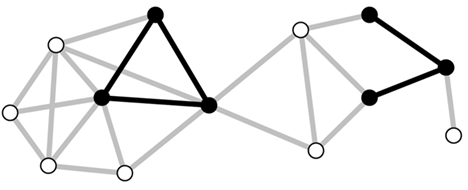
\includegraphics[width=0.4\textwidth]{%
      img/Sporns2011_Fig1C.png} %
    \nocite{Sporns2011}
  \end{figure}


  \begin{center}
    \Large Bernstein Conference 2018 Satellite Workshop:\\
    \textit{Adaptivity and Inhomogeneity in Neuronal Networks}
  \end{center}

  \vspace{0.2cm}
  
  \begin{figure}
    \centering
    
\includegraphics[width=\textwidth]{%
      img/logo_banner3.png} %
  \end{figure}



\end{frame}

